\documentclass[journal]{vgtc}       % preprint (journal style)

%% Uncomment one of the lines above depending on where your paper is
%% in the conference process. ``review'' and ``widereview'' are for review
%% submission, ``preprint'' is for pre-publication, and the final version
%% doesn't use a specific qualifier. Further, ``electronic'' includes
%% hyperreferences for more convenient online viewing.

%% Please use one of the ``review'' options in combination with the
%% assigned online id (see below) ONLY if your paper uses a double blind
%% review process. Some conferences, like IEEE Vis and InfoVis, have NOT
%% in the past.

%% Please note that the use of figures other than the optional teaser is not permitted on the first page
%% of the journal version.  Figures should begin on the second page and be
%% in CMYK or Grey scale format, otherwise, colour shifting may occur
%% during the printing process.  Papers submitted with figures other than the optional teaser on the
%% first page will be refused.

\usepackage{mathptmx}
\usepackage{graphicx}
\usepackage{times}
\usepackage{caption}
\usepackage{color}
\usepackage{bm}
%\usepackage{svg}
\usepackage{amsmath}
\usepackage{amssymb} % use this for \mathbb 
\usepackage{microtype}
\usepackage[normalem]{ulem}
\usepackage{hyperref}
\usepackage{footnote}
\usepackage{adjustbox}


\newcommand{\todo}[1]{\textcolor{red}{\textbf{TODO:} #1}}

% following commands are 'non standard' and not bundled with template, delete it problems occur
\usepackage{xargs}                      % Use more than one optional parameter in a new commands

% REDMINER:
%\usepackage[pdftex,dvipsnames]{xcolor}  % Coloured text etc.




%TODO: modified caption setup
%\captionsetup[table]{justification=justified,singlelinecheck=false}
\captionsetup[figure]{justification=justified,singlelinecheck=false}

\vgtcinsertpkg



\title{\textsc{Comvi} - Comparative Visualization of Molecular Surfaces using Similarity-based Clustering}

\author{Wilhelm Buchm\"uller, Shoma Kaiser, Damir Ravlija, Enis Spahiu}
\authorfooter{
\begin{tabular}{cc}
 Wilhelm Buchmüller  & Shoma Kaiser \\
 \href{mailto:buch.willi@googlemail.com}{buch.willi@googlemail.com}     & \href{mailto:shoma.kaiser@googlemail.com}{shoma.kaiser@googlemail.com} \\
 Enis Spahiu & Damir Ravlija  \\
 \href{mailto:enis.spahiu@hotmail.de}{enis.spahiu@hotmail.de} & \href{mailto:st144386@stud.uni-stuttgart.de}{st144386@stud.uni-stuttgart.de}

\end{tabular}
}



%other entries to be set up for journal
%\shortauthortitle{Schmid \MakeLowercase{\textit{et\,al.}}: ProjINF for fun and profit}


\abstract{
The goal of this paper is to show the reader the abstract methods and concrete applications that were used to cluster the proteins by similarity. We built a plugin MSMCLUSTER for MegaMol framework that visualizes the results of clustering in a novel way. As representations of protein surfaces we used Molecular Surface Maps that were provided by Krone et al. \cite{molecularmaps}. To extract the features from Molecular Surface Maps image moments were used. Using the extracted features we clustered the data using different clustering algorithms like K-means and hierarchical agglomerative clustering. To visualize the data we used representative images of clusters in a force directed layout. To further enable the user to analyze the results of clustering ability to perform and visualize the clustering one level deeper was included.  Since the researchers might work with large data sets, plugin was extended in order to include possible interactions with large high-resolution display Powerwall.  In order to test the clustering results we created three different data sets of Molecural Surface Maps from  Solvent Excluded Surfaces of proteins. We compared the results of different clustering algorithms applied to those data sets. The paper describes the process and the approaches that were taken to solve these tasks. 

} 


\keywords{Clustering, Dimensionality Reduction, ssstSimilarity, Feature Extraction, Visualization, Large High-Resolution Display, MegaMol}

%% ACM Computing Classification System (CCS).
%% See <http://www.acm.org/class/1998/> for details.
%% The ``\CCScat'' command takes four arguments.

\CCScatlist{ % not used in journal version
	\CCScat{Computer Graphics}{I.3.8}{Applications}{Molecular Dynamics Visualization}
	\CCScat{Simulation and Modeling}{I.6.6}{Simulation Output Analysis}{Molecular Dynamics Visualization}
	\CCScat{Computer Graphics}{I.3.7}{Three-Dimensional Graphics and Realism}{Raytracing}
}

\graphicspath{{pics/}}

% Uncomment below to include a teaser figure.
\teaser{
\centering
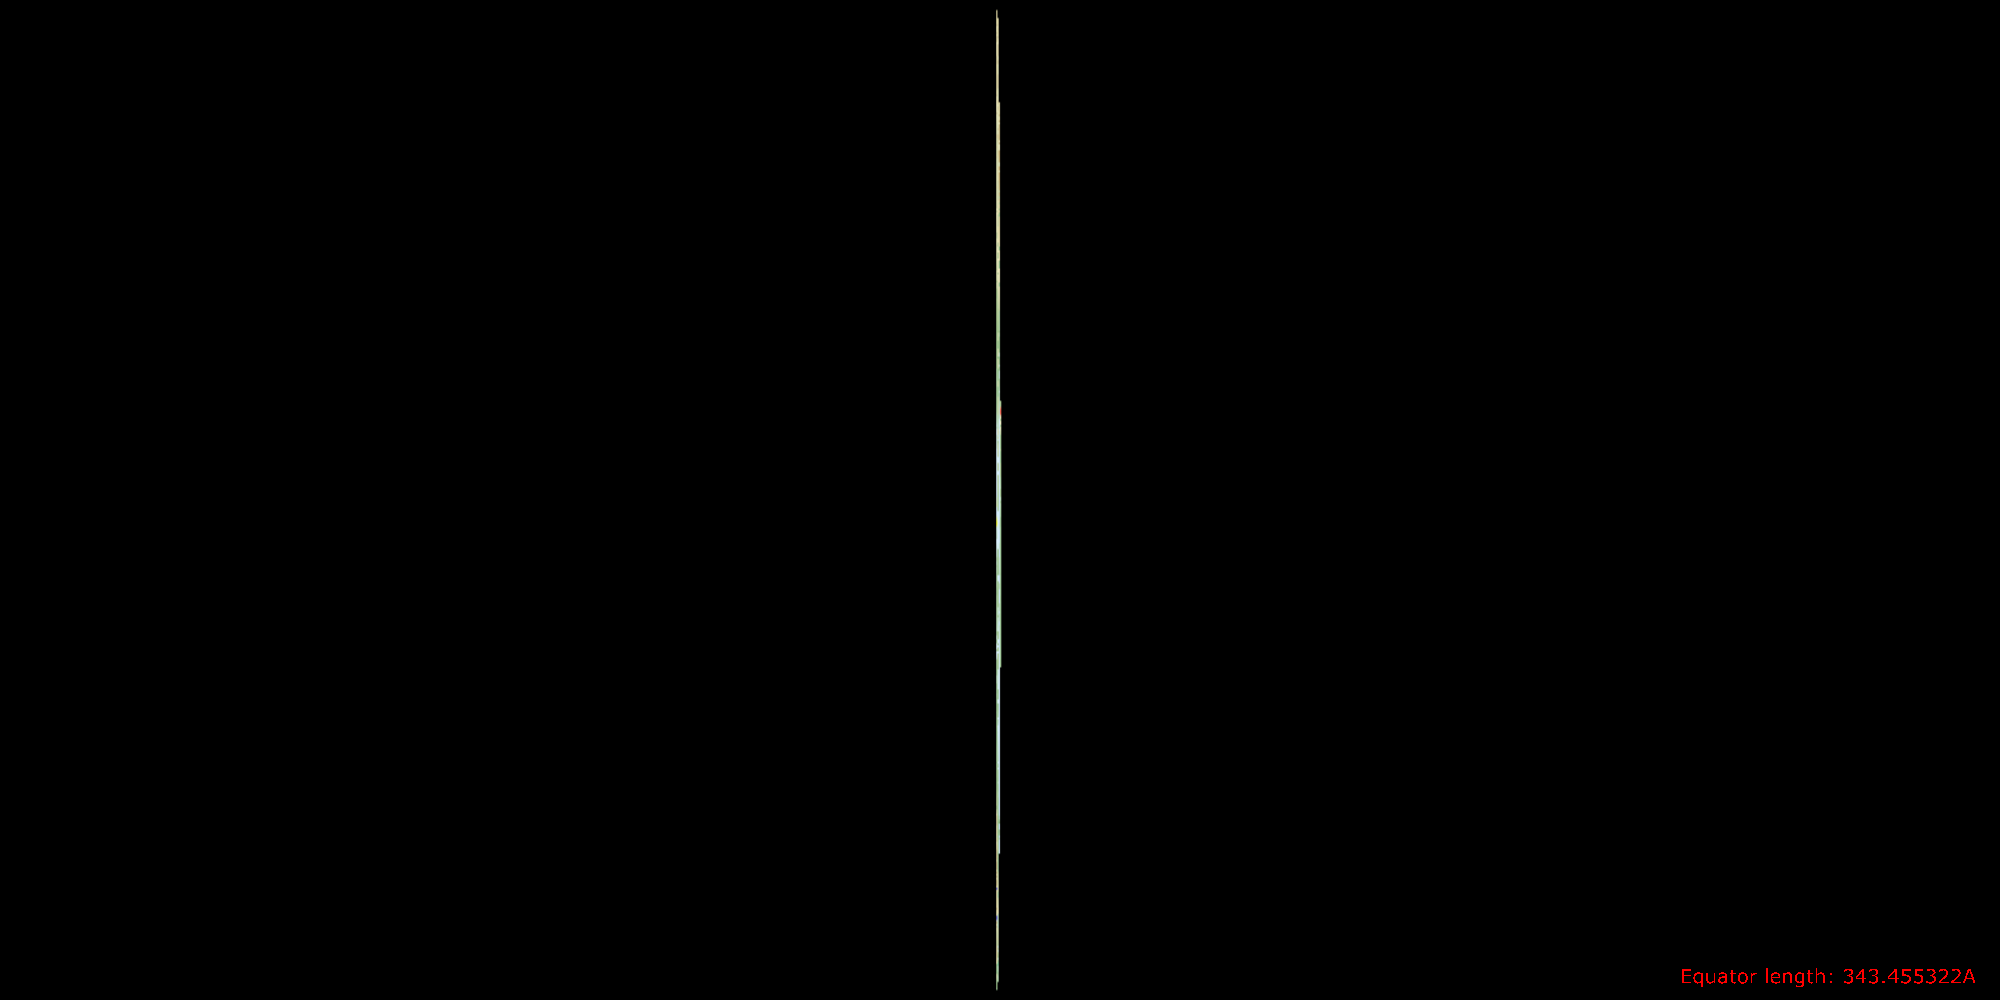
\includegraphics[width=12cm]{teaser.png}
\caption{Screenshot of a running MegaMol/\textsc{MSMCLUSTER}/comvi instance 
}\label{fig:teaser}
}

%%%%%%%%%%%%%%%%%%%%%%%%%%%%%%%%%%%%%%%%%%%%%%%%%%%%%%%%%%%%%%%%
%%%%%%%%%%%%%%%%%%%%%% START OF THE PAPER %%%%%%%%%%%%%%%%%%%%%%
%%%%%%%%%%%%%%%%%%%%%%%%%%%%%%%%%%%%%%%%%%%%%%%%%%%%%%%%%%%%%%%%%

\begin{document}

%% The ``\maketitle'' command must be the first command after the
%% ``\begin{document}'' command. It prepares and prints the title block.

%% the only exception to this rule is the \firstsection command
\firstsection{Introduction}\label{sec:intro}
%
\maketitle
%
\firstsection{Introduction} 
%\todo{add sections to tasks in this section}%for journal use above \firstsection{..} insteadsss
Over the span of the last 6 months we  have researched and implemented a comparative clustering  process for images of molecular maps.
The task consisted of several parts: to generate Molecular Surface Map images with the existing \verb|molecularmaps| plugin for MegaMol \cite{MegaMol}, to build up a data set, to extract a descriptive feature vector from the image, to find a way to cluster the extracted  feature vectors by similarity  and to visualize the resulting clustering on the large high-resolution display ``Powerwall''. The interaction with the Powerwall was to be done with  an existing tracking device.

The result of this work is an \verb|MSMCLUSTER| plugin that  extends the functionality of the MegaMol\cite{MegaMol} visualization framework. \verb|MSMCluster| contains two modules that cluster Molecural Surface Maps and visualize the results of the clustering. ClusterRenderer module visualizes the clustering using the force directed layout and in ScatterPlotRenderer individual images are represented as points in two-dimensional space and allow the user to see the distances between images.

MegaMol is a simulation tool developed by the Universit\"at Stuttgart and the TU Dresden. It can be used to visualize particle data, simulations on atomic scale and other molecular processes such as the one that we are presenting with our work. 
Due to its modular nature, it can be extended with modules to either build standalone plugins or build modules that interact and interface with each other.
In this paper we guide you through the \verb|MSMCLUSTER| plugin, its capabilities and inner workings.

The first task was to retrieve molecular image data through existing MegaMol plugins \cite{molecularmaps}. For this a special binary of megamol was compiled and will be released in a separate project that will be publicly available starting \today \footnote{\url{https://github.com/aiosin/comvi}\\ Last retrieved: \today}.
The next task was to extract an expressive feature vector from those images and to find a metric to cluster them by similarity.

The last task which was also developed in a plugin in MegaMol was the visualization on the VISUS Powerwall. The Powerwall is a very high resolution display \footnote{\url{https://www.visus.uni-stuttgart.de/institut/visualisierungslabor/technischer-aufbau.html} \\ Last retrieved: \today } that can be used to visualize large data(sets). Due to its size and resolution it is possible to display much more information than on a regular consumer grade screen. 

The Powerwall supports a tracker device that can transmit 6 degrees of freedom, so for the interaction step we had more possibilities than with traditional human interface  devices  (HIDs), aside from devices like modern smartphones. For this last step we also researched the possible interactions with the unique tracking device  which can be used to interact the Powerwall.

The task required from us that we learn how to compare the images, measure the similarity  distances between the images, and cluster them. Further it  required that we use a similarity based clustering algorithm.
% added here to make it appear on the second page
\begin{figure*}[htbp]
	\begin{center}
		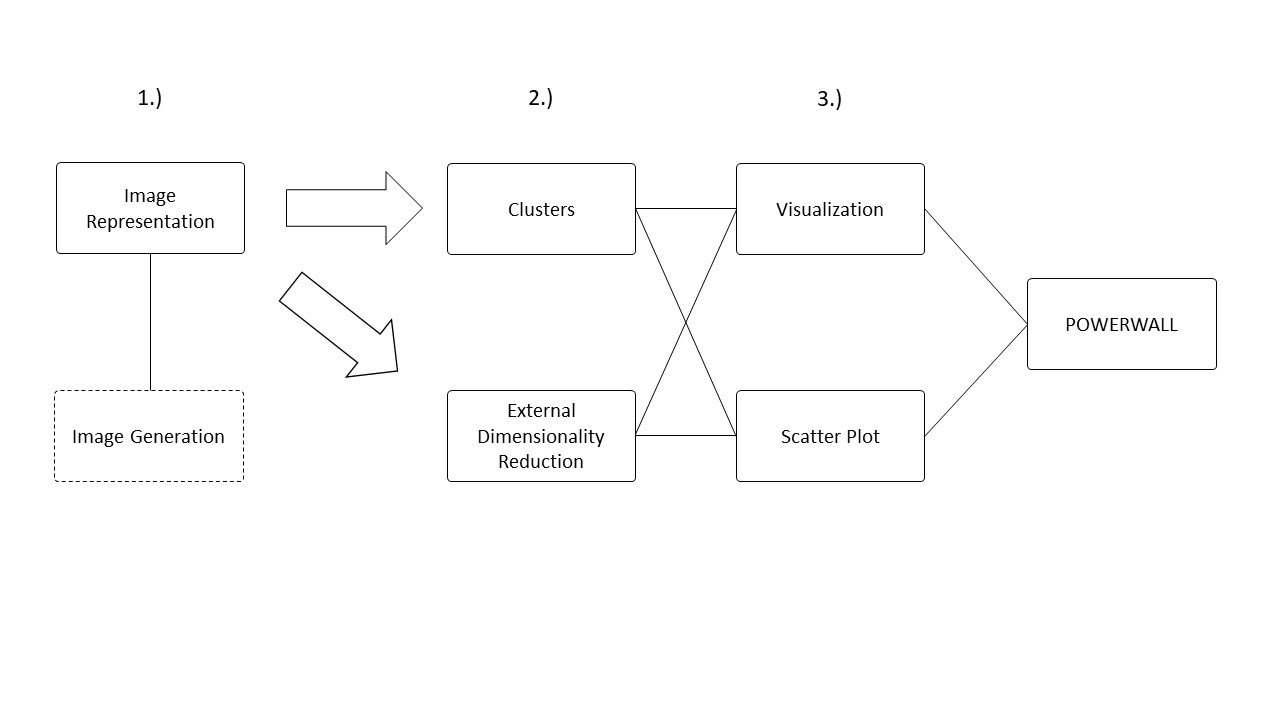
\includegraphics[width=.75\linewidth]{Folie1}
	\end{center}
	\caption{\label{fig:arch} Architecture of the system that was implemented in comvi and MSMCluster.\todo{replace with vector graphic}}
\end{figure*} 
%Initially we were given the choice, we could either choose to find similarities between the proteins and cluster the proteins jin the \verb|.pdb| format or using bitmap image generated by the \verb|MolecularMaps| plugin in MegaMol \cite{molecularmaps}.

%Since handling image files, which give information about the protein in two dimensions was easier than dealing with the \verb|.pdb| file format which results in three dimensional structures, we decided to start and carry out the task with the two dimensional approach. Kolesar et al. discuss the advantages of comparing and visualizing of proteins with their Molecular Surface Maps \cite{kolesar}.


To prevent confusion further down the paper  the reader should be familiar with the following two terms: \textsc{Comvi} - internal name of the clustering engine that can be used by the MegaMol Plugin \\
\verb|MSMCluster| - name of the Megamol plugin that was developed as the main part of the project.

Over the course of the next few pages you will learn how we approached these challenges and how we (attempted) solved them. You will find out what  worked and what didn't. In the second chapter related work is presented. Chapter three is the main part of the paper and shows our approaches to clustering and extracting features from the protein images that were used in the clustering. In chapter four our approaches to the visualization of data on conventional desktop computers and large high-resolution displays In this chapter we also describe shortly \verb|MSMCluster| plugin and discuss its strengths and limitations. In chapter five we present and discuss the results of applying MSMCluster plugin onto data sets of different sizes. In the end in the conclusion we shortly discuss possible future work.

%-------------------------------------------------------------------------

\section{Related Work}\label{sec:relatedWork}

Clustering proteins by similarity or comparing individual proteins has been subject of existing work.

The paper ``Unfolding and interactive exploration of protein tunnels and their dynamics'' \cite{kolesar} from Kolesar et al.  already had similar approaches to ours. Kolesar et al. used a 10 dimensional feature vector based on invariant image moments defined by Hu \cite{humoments}. Hu-Moments are set of invariant moments defined over a two dimensional signal, that give unique features about the the object in the image. More about image moments and the Hu Moments in section \ref{subsec:humom}.


Another approach for 3D protein data were 3D Zernicke moments explored by La et al. in \cite{3dsurfer}. The approach is basically the same as in Kolesar et al. but La et al.  in \cite{3dsurfer} used Zernicke moments instead of traditional image moments and extended them to three dimensions. More about the comparison of the different methods in \ref{subsec:comparison}.
 

For further information and more complex approaches to this problem one should consult the Smith Waterman algorithm \todo{mail: expand} from Smith and Waterman ``Identification of Common Molecular Subsequences''\cite{smithwater}. This work consideres the protein as a one-dimensional sequence of amino acids, rather than extracing two or three dimensional features over a two or three dimensional signal.\footnote{An overview can be found here: \\ \url{https://www.ebi.ac.uk/Tools/sss/}\\ Last retrieved \today}ss

Visualization of data on large high-resolution displays was discussed in Müller et al. \cite{powerwall}. System that they build could be used on large high-resolution displays as well as consumer grade desktops and allowed comparison of simulation results. They also conducted a user study where the participants could compare different views of the protein in the simulation. They had to choose the view that was closest to the baseline. Their results showed that depending on the data set, users were either more precise and also more confident that they found the correct solution when using large high-resolution ssdisplays, or users had the same precision and confidence as when they used visualization on conventional displays. System used for the user study was showed to the experts in the field of technical biochemistry as well. They said that this way of visualizing the data would possibly allow new discoveries in some areas of their research.
\section{Clustering}
%\todo{write some intrduction to clustering, aufteilen in subsections}

%\todo{this will be the main section for the clustering topic }
Due to the given generated data  not being  labeled, only unsupervised machine learning techniques like clustering could be applied on it. 
Clustering of data is defined as the process of grouping $n$ distinct values into $m \leq n$ different classes. Clustering algorithms are algorithms that perform clustering. They can be subdivided in two different ways \cite{iir}.

Depending on the number of classes to which one data point can belong, one can differentiate  between hard and soft clustering. In hard clustering one element can belong to only one class, whereas in soft clustering it can belong to many different classes.
On the other hand, depending on the way in which the data is clustered one can differ between flat and hierarchical clustering. In flat clustering particular clusters have no relation to each other, whereas in hierarchical clustering one considers the distance between clusters as well, resulting in a hierarchy.


\subsection{Approaches to the Clustering-Problem}

At the start of the project we had several ideas of how we could approach this problem. 
Trying to follow the recent trend in machine learning we researched possible ways to incorporate neural networks to compute a simlilarity metric between  two images or classify an image into a more usable vector of data.

We ended up using a higher dimensional feature vector described in section \ref{sec:featurev} to  compute the similarity between two protein maps because we didn't manage to train a custom neural network model in the given timeframe, partly due to lack of knowledge in the field of machine learning and also due to the lack of labeled data, which would have been required.

If one had labeled data, one could easily train an autoencoder, SVM or simple neural net (if the number of classes is relatively low).

Our relatively spartan results with a pretrained Imagenet \cite{imagenet}\footnote{\url{https://pjreddie.com/darknet/imagenet/} \\ Last retrieved: \today}  model led us to believe that given the knowledge on the subject, and  data labeled by the human experts or algorithms (based on known features or descriptors) in that field or   it should be possible for this specialized task to find a machine learning  solution using neural networks/autoencoders.



\subsection{Finding a feature vector to cluster the images}\label{sec:featurev}

This section describes the process of finding a feature vector that describes the  Molecular Surface Maps. Some of those feature vectors were then used as an input to the clustering algorithms used by the  \verb|MSMCLUSTER| plugin (see  Figure \ref{fig:arch}).

The challenge of finding a good feature vector is to find good features which can give a lot of information about the image.
If the extracted image features are bad, that is they do not describe the images in a useful way, the dimensionality reduction will give noisy results and the clustering algorithms will not group the images in any meaningful way, so users will not be able to extract any new information from the clustering.

The following procedure after finding the feature vector for a given image is to apply some sort of dimensionality reduction to project a higher dimensional vector onto a 2D or 3D space.

This has multiuple advantages one of which is that if the dimensionality reduction works as intended one can easily find out after applying the dimensionality reduction if similar looking items are positioned next to each other.

\subsubsection{Curse of dimensionality}
Alternatively one could also find a similarity measure for higher dimensional vectors, but this problem has turned out harder than it seemed partly due to the \textit{curse of dimensionality}\footnote{\url{https://www.inf.fu-berlin.de/inst/ag-ki/rojas_home/documents/tutorials/dimensionality.pdf}\\ Last retrieved: \today}.


Contrary to expectations, on very high or infinite dimensional spaces, unexpected things start to happen. If we  such as the euclidean distance or mathematically put the \(L_2\)-norm loses relevance since
\begin{equation}
\lim_{n\rightarrow \infty} x^n = 0 \quad \forall x \in [0,1)
\end{equation}

Simply put, otherwise very dissimilar values have their distance drawn to zero. For example between a vector with \(0.99\) in every dimension and a vector with \(0\)in every dimension the eucludian distance is: \(0.99^{100} = 0.33660\) which would put them closer than one would assume them to be.

So we have to come up with other solutions to this problem discussed in section \ref{subsec:dimred}. % TODO: maybe subsec:simmes ???

After looking at a small subset of molecular map images from a variety of proteins we assumed that we could  extract feature information about the following properties of a given image: 
\begin{itemize}
  \item Color distribution
  \item Shape
  \item Texture
  \item Invariant  Image Mmoments 
\end{itemize}


The initial idea was that the color distribution gives information about the color palette and local color changes in the image, the extracted shape features should give information about the the biggest \( n \) shapes in the picture, the texture feature should differentiate between smooth and rough and coarse texture and everything in between.

The image moments were chosen as a goto approach to extract invariant features from the image which has been proved to yield usable results as described in Kolesar et al. \cite{kolesar}.

The exact image features that we extract from the image are the following:
\subsection{Image Features/Descriptors}
This section explains the different image features that we used to build the feature vector.
For the length of this section the reader must know that we rescale all images to the size of $(128,128)$ after reading them into our routine.
\subsubsection{Invariant Image Moments by Hu}\label{subsec:humom}

The set of invariant Image Moments discovered by Hu et. al  are rotation, translation, scale and transformation  invariant. This allows us for example to determine if an image $I_a$ is similar to another image $I_B$ if $I_B$ is equal to $I_A$ and simply rotated by $30^{°}$.

The continuous  Image, defined over the domain \(\mathbb{R}^2\) Moments  over two dimensions at their core are defined as such:

\[M_{p,q} = \int^\infty_{- \infty}\int^\infty_{- \infty} x^py^q f(x,y) dy dx \]

Where \(f(x)\) is the signal of the image.  

When dealing with discrete values like we find them in a discretized RGB or greyscale (GS) image, we use sums instead of integrals, so we get the following formula:

\[M_{i,j} = \sum^n_{i=0}\sum^m_{j=0} x^i y^j f(x,y) \]

%TODO: damir add this 
Kolesar et al. ended up using a collection of 10 experimentally determined moments to cluster the image. In our case the moments we used the standard Hu et al. invariant moments. 

To define the images internally in MSMCluster plugin we used image moments that were defined by Kolesar et al. They represented grayscale images using 10 dimensional vectors. 

\subsubsection{Color palette/histogram }

The goal when extracting color palette was to reduce the big color space that is present in any of the molecular maps and get a few distinct  colors that describe the color space with a few representative colors.

To achieve this we extract a histogram of each color channel of the RGB images. Each channel is then represented as a greyscale image. We then create for each channel a histogram of the luminance intensities with in our case 16 bins. This ``reduces'' the \(128*128 = 16.384\) dimensions to just \(48\) dimensions for our image.

An alternative approach we had to extract color information about the image is to split the image in to equally sized chunks and to extract simple color distribution features like average, min and max values.

The results from both approaches will be discussed in \ref{subsec:dimred}.

\subsubsection{Texture}
%\todo{better introduction}
After looking at the smallest data set of molecular maps we noticed that many samples had a distinct roughness that looked like they could be used to classify their texture.

We ended up using the Haralick textural features \cite{haralick}  . The Haralick features work with a grey level correlation matrix (GCM). The GCM for a given greyscale image is defined as such:

\[{\displaystyle C_{\Delta x,\Delta y}(i,j)=\sum _{x=1}^{n}\sum _{y=1}^{m}{\begin{cases}1,&{\text{if }}I(x,y)=i{\text{ and }}I(x+\Delta x,y+\Delta y)=j\\0,&{\text{otherwise}}\end{cases}}}\]

The Haralick features compute, based on this matrix, features that aim to describe the texture of the original source image.

The features include eg. the angular second (image) Moment, entropy, sum variance/energy/average.\footnote{\url{http://murphylab.web.cmu.edu/publications/boland/boland_node26.html} \\ Last retrieved: \today}

Also we can take more features from that GCM which gives us more features to work with.\footnote{\url{http://murphylab.web.cmu.edu/publications/boland/boland_node26.html} \\ Last retrieved: \today}

We also computed this on every channel yielding us \(3 \times 14 \) features.

Alternatively one can also use the  texture features developed by Tamura et al.  in ``Textural Features Corresponding to Visual Perception''\cite{tamura}. The Tamura features are different to the Haralick featues since they were developed on a basis of psychological experiments. The Tamura features do not use a GCM, instead they used a combination of kernel convolutions that yield  the information about the coarseness, contrast, directionality, linelikeness, regularity and roughness.

\subsubsection{Shape}
We did not end up using the shape features described here but, since we spent quite some time researching this problem, I think it is important show how and why they were created.

The shape features we hoped to use were  fourier descriptors\footnote{\url{http://fourier.eng.hmc.edu/e161/lectures/fd/node1.html} } \footnote{\url{http://demonstrations.wolfram.com/FourierDescriptors/}}. In short, we get the centroid-distance curve of a distinct shape and take the fast (discrete) fourier transform of that curve. The technique has been proven to work for shape recognition  in earlier works \cite{fourierd}.  

Our approach was the following.  Since our molecular maps are extremely complex (image-wise) we first need to divide the image into discrete image region.  We preferably want to segment our image into $n$ colors. To recap: our everyday monitor does support \(24\) bit colors, \(8 \) bit per channel. This gives us \(2^{24}=16.777.216 \) total colors.
To find a valid contour in that colorspace would be a coincidence in most cases.
So our approach is to compress the color space down to a couple of colors.
This proces is called color segmenatation. We use the k-means algorithm to put every color from our original image into a few bins.

Alternatively the mean-shift algorithm can be used. The algorithm is a kernel based clustering algorithm which operates sort of like the gradient descent algorithm. The mean shift algorithm is explained in detail in section \ref{sec:clusteringa}.
Each point has a weight and initally all the points are laid out on a grid (or your dimensions next best spatial representation) each value attracts with a constant force all other neighboring values so they all suck each other in discrete clusters depending on the parameters (bandwith size and kernel weight). 

A comparison of color segmentation of mean shift and  k-means can be seen here\footnote{\url{https://spin.atomicobject.com/2015/05/26/mean-shift-clustering/}} 
\footnote{\url{https://spin.atomicobject.com/2016/12/07/pixels-and-palettes-extracting-color-palettes-from-images/} \\ Last retrieved \today}. 


But our problem of color segmenatation was stil not solved. Especially in the k-means algorithm we encountered a lot of smaller ``irrelevant'' shape artifacts that we did not want.
So one way of getting them out of the way was to squash the color space further down to two or three distint colors in the image.

The other way is to  dynamically (depending on each image) dilate and erode \footnote{\url{https://docs.opencv.org/2.4/doc/tutorials/imgproc/erosion_dilatation/erosion_dilatation.html}\\ Last retrieved \today}the image until we can detect with a matrix labeling  or   floodfill algorithm that we really have only a handful of shapes in the image.

For the shapes we then extract the contours and compute the centroid of that shape.
The centroid is the geometric center of mass of the image which can be built up by the first central moments of the two dimensions.

Now we have the centroid and the contour of the shape that we want to classify we need to form the contour centroid distance curve.
The contour centroid distance curve is simply a disrete list of values of the \(x\)and \(y\)  values of each item of the contour  or alternatively the list of the euclidian  distances from the centroid, both approaches have been shown to work.

We then normalize the values by diving all the values by the biggest value in the array, resulting in a array that is in range $(0,1]$.

Without loss of generality depending on which curve we chose we take the fast discrete fourier transform of that signal, which gives us for each sine/cosine coefficient a weight how that component contributes/weighs in the signal.

Without any proof that would go beyond the scope of this paper we can say that the gained features are rotation scale and translation invariant. It is rotation invariant because the Fourier transform is shift invariant so it does not matter where we begin our centroid curve; the power spectra of the Fourier transform will be the same even if its rotated. Its scale invariant because we normalize it and it is translation invariant because the distance curve itself is  translation invariant.

Another shape feature can be won, under the condition that the shape object is given as a greyscale binary matrix. From this matrix one can extract Image Moment features like the one by Hu as described in section \ref{subsec:humom}.

We did not end up using the shape features, because we could not notice any improvement over the other features that we used, but we put substantial effort into getting these features to work, so we wanted to describe our process here.

% \subsection{Finding the best performing similarity measure}\label{subsec:simmes}

% After our feature processing on an image we end up with an feature matrix where the rows are samples  and the columns are the features.  \[A \in \mathbb{R}\] \todo{remove (?) }


\subsection{Finding the best performing  dimensionality reduction method}\label{subsec:dimred}
For testing purposes we used every dimensionality reduction method we could find that looked halfway promising. We tested on data sets of various sizes and content.

We tested our results on the medium sized Oxford flower data set\cite{flower}, the large sized car  \cite{stanfordcar}data set and our large ($\sim$3600 images) molecular maps data set. 
We further extracted a smaller sized ($\sim$300 images) data set as our benchmark set  and an easy to benchmark and a small (12 images) data set for faster testing. 

As you will find in our comvi repository \footnote{\url{https://github.com/aiosin/comvi}} the dimensionality reduction routine consists of passing it a feature array of shape \(A^{n\times m}\) where \(n\) is the number of samples (i.e. the number of images) and \(m\) is the number of features per sample.
In the routine we additionally scale the data because we want to avoid potentially unwanted effects caused by very big feature values.\footnote{\url{https://medium.com/greyatom/why-how-and-when-to-scale-your-features-4b30ab09db5e} \\ Last retrieved: \today}
We then return the reduced feature array back to the callee. The callee can then apply further some functions on this reduced array.

After inital testing with linear dimensionality reductions we notice that our results just wouldnt ``converge'', so we again tried with any non linear dimensionality reduction technique we could find.

We tested our data with Local Linear Embedding (LLE), Multi-Dimensional Scaling (MDS), Kernel-PCA, Isomap and t-distributed Stochastic Neighbor Embedding (t-SNE).
After testing with a small non representative user group that would judge how good the clustering was done by the technique we concluded that t-SNE performed the best.

Further testing leads us to believe that t-SNE is the best dimensionality reduction procedure for this problem. t-SNE is discussed in more detail in section \ref{sec:clusteringa}


\subsection{Clustering - Algorithms and strategies }\label{sec:clusteringa}
We applied the following clustering algorithms to image descriptors that were extracted from the protein images.

\begin{description}
\item [K-means] takes the number of clusters as an input and if the data set contains more elements than the wanted number of clusters groups elements into that many clusters. Since it always groups data into the specified number of clusters, K-means is a flat clustering algorithm. Owing to the fact every image is clustered into only one cluster it belongs to hard clustering algorithms. 

To cluster the data K-means uses the concept of centroids. A centroid is a point in vector space that is located in the middle of the corresponding cluster. There is therefore one centroid for every cluster. 
At first K-means initializes the same number of centroids the same as the number of clusters. This can be done by choosing randomly $k$ samples  in the vector space. Since K-means is an iterative algorithm  it then repeats reassignment and recomputation steps until it minimizes the distance between the centroid and all of the elements of the corresponding cluster as follows \cite{KI17}: 

Let $D = \{x_i\}_{i=1}^n$ be a set of $n$ vectors $x_i$ that represents some data. This data should be clustered into $k$ clusters whose centroids are  $\mu_{c(i)}$. Now let $c: i \mapsto k$ be the assignment of the element $i$ to the cluster $k$. 
K-means minimizes the following loss function $L$:
\begin{equation}
\label{form: loss}
L = \min_{c, \mu} \sum_{i=1}^{n}(x_i - \mu_{c(i)})^2
\end{equation} 
This minimization is done by repeating the reassignment (\ref{form:reassignment}) and recomputation (\ref{form:recomputation}) step.
\begin{equation}
\label{form:reassignment}
\forall i: c(i) := \operatorname*{arg\,min}_k (x_i - \mu_k)^2
\end{equation}
\begin{equation}
\label{form:recomputation}
\forall k: \mu_k := \frac{1}{|c^{-1}(k)|} \sum_{i \in c^{-1}(k)} x_i
\end{equation}


The main weakness of K-means is that it does not converge to a global minimum. In order to circumvent this problem centroids are usually initialized randomly, but makes  the algorithm non-deterministic. To find the best possible clustering  several restarts of the algorithm are  sometimes needed.  Another disadvantage is that K-means finds only spherical clusters because it adds an image only to the cluster whose corresponding  centroid is nearest to it \cite{jain2010data}. The main advantages of K-means  on the other hand are that it often gives good results and is easy to implement. It is also efficient because its time complexity is linear in the number of elements, number of clusters and number of iterations. 

The \verb|MSMCluster| plugin contains two implementations of K-means. We implemented one version ourselves and the other version is part of the dlib library \cite{dlib09}.
\item [Hierarchical agglomerative clustering] is a type of hierarchical clustering that clusters the data from the bottom up. As an input it takes the wanted number of clusters. It starts by making a cluster for every element in the data set. Then repeatedly merges clusters that are the most similar according to some metric until in the end there is only one cluster left. However in the course of every merging operation it takes a note of the similarity between the clusters that are merged. This way it builds cluster hierarchy that can be visualized with dendrograms\footnote{A dendrogram (from Greek dendro "tree" and gramma "drawing") is a tree diagram}. The given number of clusters is then obtained by cutting the tree on the right similarity level. This is done by descending from top of the tree and taking into account the number of siblings on every similarity level \cite{iir}.

Main advantages of hierarchical agglomerative clustering is the hiararchy of clusters that it creates, and its stabililty over multiple executions of clustering. Its main weakness is on the other hand high time ($O(n^2 log(n))$) and space complexity ($O(n^2)$) \cite{jain1999data}.

The \verb|MSMCluster| plugin uses implementation of hierarchical agglomerative clustering that is contained in the dlib library. 
\item [Mean-shift] is another clustering algorithm that uses the concept of centroids \cite{dlib09}. %TODO: expand
\end{description}

\subsection{Finding the best performing clustering algorithm}
Our approach to finding a clustering algorihtm was the same as the one that we used  to find the best performing dimensionality reduction algorithm.

Except with a little modification. Kolesar et al. \cite{kolesar} used the k nearest neighbors algorithm over their 10-dimensional feature vector to cluster their data, as they discuss their results. We decided to further use this approach to cluster our molecular maps instead of the molecular protein tunnels which Kolesar et al. analyzed.


In the early stages of the projcet we intended to use the DBSCAN clustering algorithm. 
The key feature to this algorithm is that it automatically determines the optimal number of clusters that it detects in the given data. 

The algorithm is a density based spatial clustering algorithm that uses a similarity metric between two items that are to be  clustered defined over the domain \([0,1]\). So the ways of computing the similarity is given more freedom with this approach.

You could use the euclidian distance between two feature vectors, the cosine distance or feed the two images to a siamese neural network/autoencoder. Siamese neural network are, for the sake of simplicity, two identical black box oracle machines which yield different valued vectors if you feed the two machines two different signals and  an autoencoder is a machine which will have learned to classify data into a few distinc categories. The main disadvantages two both of these techniques is that both the siamese neural network and the autoencoder have to be trained. 

You could also use the Haussdorff distance to compare two higher dimensional vectors. A detailed explanation would go beyond of the scope of this paper, but the the Haussdorff distance is simply put the ``maximum distance of a set to the nearest point in the other set''\footnote{\url{http://cgm.cs.mcgill.ca/~godfried/teaching/cg-projects/98/normand/main.html}}.

We opted against DBSCAN for our primary clustering algorithm because in the early stages of the project the computation of the \(n\times n\) similarity matrix was  computationally expensive and took more time than the approaches that we demonstrate in the next paragraphs.

For our initial testing we used k-nearest neighbors with a preconfigured assumed number of clusters.

We further tried  a  spectral clustering  \footnote{\url{https://www.cs.cmu.edu/~aarti/Class/10701/readings/Luxburg06_TR.pdf}} and chinese whispers clustering algorithm\cite{chinesewhispers}. Both of these algorithms are graph based algorithms. The spectral clustering approach works with the eigenvalues (spectrum) of the similarity matrix (like DBSCAN), while the chinese whispers clustering does reachability analysis in a network of connected nodes.
Both of these approaches yielded unusable results, since the chinese whispers algorithm for example  is not suitable for this task and performs poorly on any similarity matrix.


We ended up with the mean shift algorithm. It also is a density based algorithm and much like the DBSCAN algorithm is also determines the optimal number of clusters for the given parameters but it operates with a kernel sampled on each point in the plot and calculates the center of mass so to speak of the points clouds\footnote{\url{https://spin.atomicobject.com/2015/05/26/mean-shift-clustering/}\\ Last retrieved: \today}. For a demonstration of the results of the mean shift algorithm look at Figure \ref{fig:tsne}. 




%\subsection{Testing the feature vector with other data sets}

\begin{figure}[tb]
	\begin{center}
		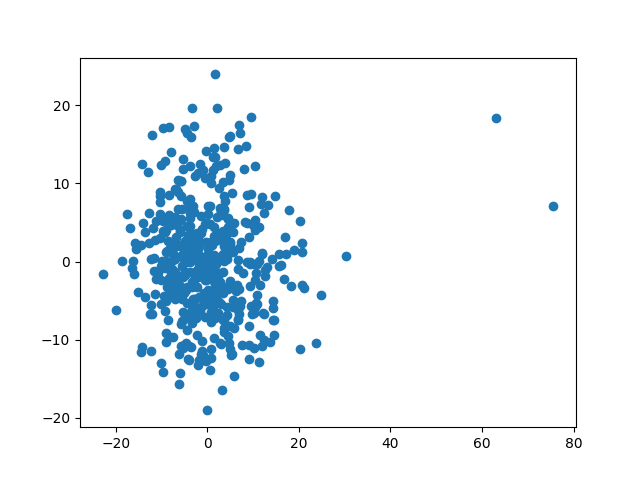
\includegraphics[width=.75\linewidth]{Figure2.png}
	\end{center}
	\caption{\label{fig:bmw} Early test with the bmw car data set }
\end{figure}
\begin{figure}[tb]
	\begin{center}
		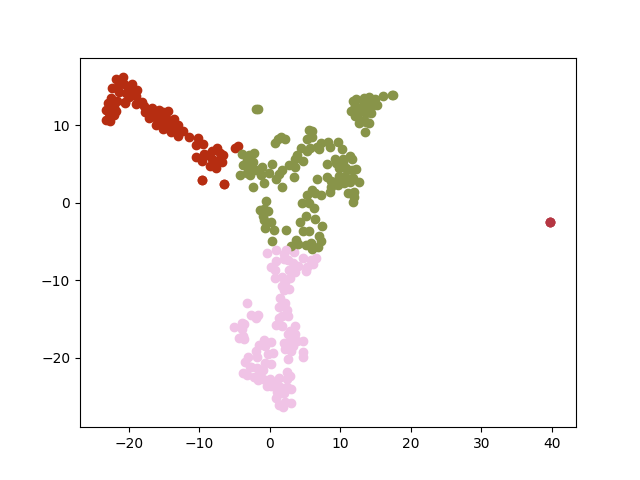
\includegraphics[width=.75\linewidth]{MS-tsne.png}
	\end{center}
	\caption{\label{fig:tsne} final test with the tsne dimensionality reduciton and the mean shift clustering algorithm }
\end{figure}

\begin{figure}[tb]
	\begin{center}
		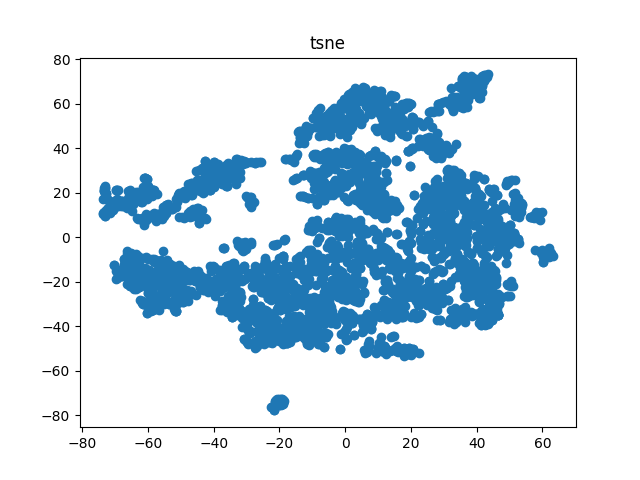
\includegraphics[width=.75\linewidth]{tsneFull.png}
	\end{center}
	\caption{\label{fig:tsnef} final test with the tsne dimensionality reduciton and the mean shift clustering algorithm }
\end{figure}

\section{Visualization and Interaction}

To show up our algorithm results, we needed a suitable representation and a intuitive interaction for our generated clusters. A tweak bar is used to   set relevant parameters like the clustering algorithm or the images to cluster.  The represented clusters are shown in a bounding box. The MegaMol application can be displayed on the previously mentioned Powerwall. A tracking device can be used to interact with the application.

\subsection{Background MegaMol and Powerwall}


The visualization of MegaMol is displayed on the Powerwall.
The  Powerwall is a merged large high-resolution display made of five portrait- oriented
strips . The setup has  a resolution of $10.800 \times 4.096 pixels$
for each eye, and is projected onto a physical screen size of about $6 \times 2.2$ metres. 
Two 4k (Liquid Crystal on Silicon) LCoS projectors are projecting the images for each strip for a total of five strips.
A pixel is about 0.56 mm  in size, which corresponds to s density of about 50 ppi.
The users interact with the system using a 6-DOF mid-air
pointing Stick with two buttons (1 on each side), which is tracked by 14 camers
using an optical tracking system. 


\subsection{Goal of Visualization and Interaction}
Afted clustering of Molecular Surface Maps, \verb|MSMCluster| plugin then visualizes results of the clustering. Both modules contained in the plugin deal with visualization of the clustering. 
%Our main goal was to find the way to visualize different clusters as clearly as possible. In order to do this, 
In ClusterRenderer \todo{reformulate} we have extracted from every cluster an image that should represent it. If the clustering algorithm used the concept of centroids, we chose the image nearest to the centroid as a representative image of every cluster. If there was no such concept, we randomly chose an image from the cluster to represent it. Representative images were then drawn onto the screen within the bounding box in MegaMol. To make the representative images fit better in the bounding box, aspect ratio of the bounding box was set to 2:1, the same aspect ratio as images.
To position the images on the screen we used techniques used from graph visualization. Every representative image was considered to be a node within an imaginary graph. To determine the positions of representative images we used the implementation of force directed graph drawing algorithm that was contained in MegaMol. Force directed algorithms are based on the physical laws and try to imitate the effect of attractive and repulsive forces on the graph nodes, as if they were connected by springs. An implementation contained in MegaMol uses repulsive forces based on Coulomb's law and attractive forces based on Hooke’s law. It also uses the concept of maximum internal energy. When internal energy becomes higher than the maximum internal energy movement of images stops. Further parameters that could be given to the force directed layout instance are damping that affects the how fast does the system calm down and integration step that defines the movement speed of the nodes. 
These parameters related to the layout were made available to the user, besides the internal energy of the top clustering level is shown to the user as well.

On conventional desktop monitors the user interacts with the 


------- 

To interact with the Application intuitively on PC and on the POWERWALL it was important that we use movements for the interactions from our everyday life. If the Application is used on PC, the MegaMol Project is mainly interacting with the mouse. If we run Application at the Powerwall it is interacting with the tracking stick.

With the four button states of the tracking sticks we focused on the most important interactions like ``selection'' or ``drag and drop'' To localize the aimung of the user  we should calculate a intersection coordinates of the tracking stick in direction to the Powerwall. While moving the tracking stick for interactions, these coordinates should be scaled for a user- friendly interactions.

\subsection{Realization}

To realize the ideas and goals we first discussed about the dimension of the cluster visualization. But a couple of reasons spoke up against a 3D visualization so we decided to do transform the 3D molecule into a 2D image. We would have more degrees of freedom to work with 3D molecules on the Powerwall. But we could not find a way to present the data in a way such that with just a glance the user could intuitively interpret the data that would be displayed on the screen. Furthermore the clustering and the interaction would be demanding. So we decided to settle for a 2D visualization. 
The visualizatoin consists of displaying the image of a cluster representative with a simple rectangle. With clicking into a rectangle the user is able to get a view of all clustered images in that cluster. Even subclustering can be executed by splitting one cluster into two more. After testing we decided that one level of subclustering is enough. After 2 levels of subclustering the clusters get too  \todo{begriff}
With the configuration bar the user is able to change several variants of clustering and execute some interactions too. 

But mainly the interactions are executed by mouse or by the tracking stick. The tracking stick got As already mentioned four states. In the first state, if no button is pressed, should be no interaction. In the second state, if the first button is pressed, should be a 'drag and drop'-interaction as we know it from the Computer. With pressing the other button, the third state, the user can select an object like we know it from the Computer 'leftclick'. If both buttons are pressed, the user is able to zoom. \todo{wenn es klappt} For the zooming we used the third dimension of the tracking area in front of the Powerwall. With walking towards the Powerwall in the fourth state the user zooms in. Equally with walking away from the Powerwall the user zooms out. 
All movements of the tracking stick in the tracking area have to be scaled for a user-friendly usage. To calculate them we tested the interactions exprimentally by changing the scalings. We adjust these parameters so that the user can operate with the whole interface without walking around in the tracking area.
As a conclusion of this part we focused on user-friendly and intuitive interactions like we know it from our everyday life.



\section{Results}
As we saw on the last few pages, we have written a plugin for MegaMol that takes a directory with generated Molecular Surface Maps as an input and clusters  them by similarity. In this section we present and discuss the results of testing three different data sets with MSMCluster plugin. 

Data sets were ordered by size and were used for different purposes. The smallest data set contained only 12 images and could therefore be used to test changes in the program quickly on all kinds of hardware. Second data set was a medium-sized data set that contained 300 images. This data set was used to test the plugin and help us notice the areas where the system needed to be optimized. The largest data set contained all of the 3600 protein images that we created. This data set will be published on Kaggle  \todo{fusnote, where?}

During the creation of Molecular Surface Maps, some of the images were not created correctly and ended up being having black areas. Those images appeared as outlying data points in scatter plots. We opted against the removal of outliers because they were often clustered into one cluster and during plugin development this proved to be a good way to test whether the clustering algorithm is working correctly.

Since there were no labeled data sets we could not use external criteria like purity or rand index to evaluate the results of our clustering. Instead we applied internal criterion of residual sum of squares to compare implementations of K-means algorithm and we also looked at the results and gave our own evaluation of them (see Table 1). We also tested the time needed to cluster and visualize the data.

\todo{discussion of the results} 



\subsection{comparing our findings with other protein similarity practices}\label{subsec:comparison}
\todo{expand} bla \cite{3dsurfer} protein database simlilarity measure.

\begin{center}
\begin{adjustbox}{max width=8.5cm}
\begin{tabular}{|l|l|l|l|l|}

\multicolumn{1}{c}{\bfseries Clustering Algorithm}  &  \multicolumn{1}{c}{\bfseries Data set} & \multicolumn{1}{c}{\bfseries RSS} & \multicolumn{1}{c}{\bfseries Evaluation} & \multicolumn{1}{c}{\bfseries Performance (in ms)} \\
\hline
K-means & \begin{tabular}{@{}l@{}}small \\ medium \\ large\end{tabular} & & & \\
\hline
dlib K-means & \begin{tabular}{@{}l@{}}small \\ medium \\ large\end{tabular} & & &  \\ 
\hline
Bottom up agglomerative & \begin{tabular}{@{}l@{}}small \\ medium \\ large\end{tabular} & & & \\
\hline
MeanShift & \begin{tabular}{@{}l@{}}small \\ medium \\ large\end{tabular} & & & \\
\hline
\end{tabular}
\end{adjustbox}
\end{center}

% \begin{table}[!h]
%   \caption{
%   \label{tab:perf} placeholder comparisons of different protein similarity comparisons/algorithms}
%   \centering
%   \vspace{0.3em}
%   \begin{tabular}{lrr}
%   data set & full performance (fps) & half performance (ms)\\ \hline\\[-0.4em]
%   big (3k images) & 1,243 & 0.1 \\
%   medium (300 image ) & 23 & 23 \\
%   small (~12 images) & 23,312,134.3 & 22.1 \\
%   \end{tabular}
%   \end{table}


\begin{figure}[h!]
	\begin{center}
		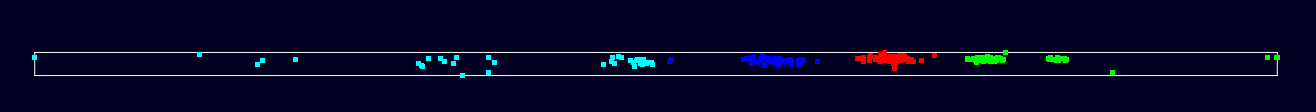
\includegraphics[width=.75\linewidth]{k-Means-mediumDataSet.png}
	\end{center}
	\caption{\label{fig:kmeans} Our implementation of K-means applied on the medium-sized data set.}
\end{figure} 
\begin{figure}[h!]
	\begin{center}
		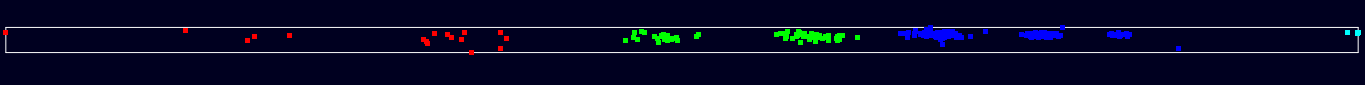
\includegraphics[width=.75\linewidth]{k-Means-dlib-mediumDataSet.png}
	\end{center}
	\caption{\label{fig:kmeans-dlib} Dlib K-means applied on the medium-sized data set.}
\end{figure}
\begin{figure}[h!]
	\begin{center}
		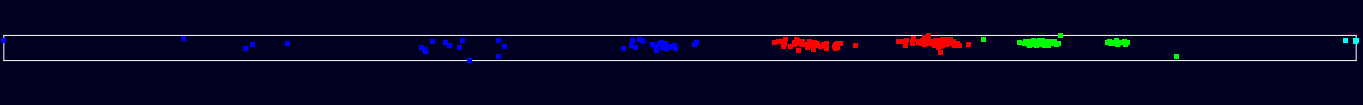
\includegraphics[width=.75\linewidth]{bottomUpAgglomerative-mediumDataSet.png}
	\end{center}
	\caption{\label{fig:bottomUpAgglomerative} Bottom up agglomerative clustering algorithm (dlib) applied on the medium-sized data set.}
\end{figure}


\section{Conclusion}
\todo{expand}
In this paper we looked at different ways of clustering proteins by similarity, visualizing results of the clustering and allowing the user to interact with the data on wall-sized high-resolution display POWERWALL. The result of our research was MegaMol Plugin MSMCluster. MSMCluster allows the user to cluster the protein images and visualize them. This plugin can be used with the Large High-Dimension Display POWERWALL. 

These Proteins were represented by Molecular Surface Maps that were extracted using the MolecuralMaps plugin.
We found that clustering results obtained with different clustering algorithms did not differ significantly, because of that we assume that further improvements in clustering of protein images might be achieved in the research of features that are extracted from the images. Perhaps further adaption of features specifically to the Molecular Surface Maps would offer further improvements of the results. 

Furthermore, with the continuation of the Moore's Law large high-resolution displays might become even more common. Because of that, further research in this area and adaptation of visualization tools and other programs to these displays might play a significant role in the future.

%% if specified like this the section will be ommitted in review mode
\acknowledgments{
We would like to thank our supervisors Michael Krone and Florian Fries as well as our project examiner Prof. Ertl, for giving us this opportunity to work on this project. We are grateful that we were able to improve our knowledge and learn new things. We are also grateful for the feedback we recieved on our work.}

\bibliographystyle{unsrt}
%%use following if all content of bibtex file should be shown
%\nocite{*}
\bibliography{comvi}
\end{document} 
